

\tikzset{every picture/.style={line width=0.75pt}} %set default line width to 0.75pt        

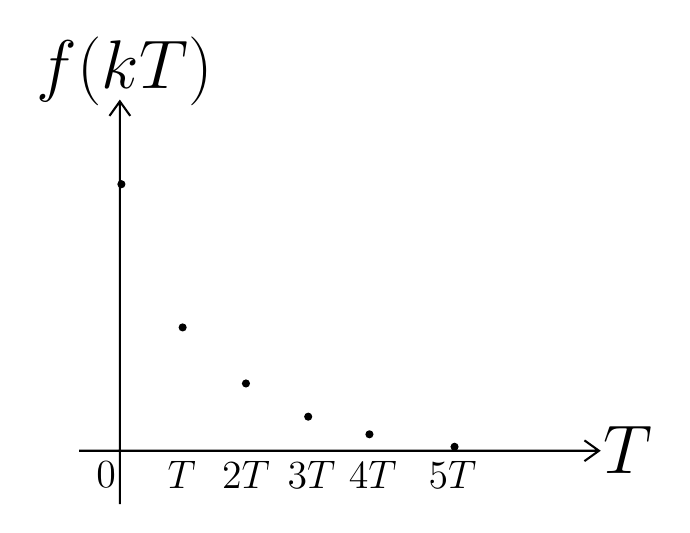
\begin{tikzpicture}[x=0.75pt,y=0.75pt,yscale=-1,xscale=1]
%uncomment if require: \path (0,300); %set diagram left start at 0, and has height of 300

%Curve Lines [id:da8133887311558856] 
%\draw    (59.67,70) .. controls (59.67,180.5) and (157.17,219.5) .. (253.17,218.5) ;


%Shape: Axis 2D [id:dp14295797745444183] 
\draw  (40,218.33) -- (290.5,218.33)(59.67,50) -- (59.67,244) (283.5,213.33) -- (290.5,218.33) -- (283.5,223.33) (54.67,57) -- (59.67,50) -- (64.67,57)  ;
%Shape: Circle [id:dp33989703923079584] 
\draw  [fill={rgb, 255:red, 0; green, 0; blue, 0 }  ,fill opacity=1 ] (88.5,158.92) .. controls (88.5,158.13) and (89.13,157.5) .. (89.92,157.5) .. controls (90.7,157.5) and (91.33,158.13) .. (91.33,158.92) .. controls (91.33,159.7) and (90.7,160.33) .. (89.92,160.33) .. controls (89.13,160.33) and (88.5,159.7) .. (88.5,158.92) -- cycle ;
%Shape: Circle [id:dp6033906991245652] 
\draw  [fill={rgb, 255:red, 0; green, 0; blue, 0 }  ,fill opacity=1 ] (119,185.92) .. controls (119,185.13) and (119.63,184.5) .. (120.42,184.5) .. controls (121.2,184.5) and (121.83,185.13) .. (121.83,185.92) .. controls (121.83,186.7) and (121.2,187.33) .. (120.42,187.33) .. controls (119.63,187.33) and (119,186.7) .. (119,185.92) -- cycle ;
%Shape: Circle [id:dp6721507659930437] 
\draw  [fill={rgb, 255:red, 0; green, 0; blue, 0 }  ,fill opacity=1 ] (149,201.92) .. controls (149,201.13) and (149.63,200.5) .. (150.42,200.5) .. controls (151.2,200.5) and (151.83,201.13) .. (151.83,201.92) .. controls (151.83,202.7) and (151.2,203.33) .. (150.42,203.33) .. controls (149.63,203.33) and (149,202.7) .. (149,201.92) -- cycle ;
%Shape: Circle [id:dp13620281514586763] 
\draw  [fill={rgb, 255:red, 0; green, 0; blue, 0 }  ,fill opacity=1 ] (59,89.92) .. controls (59,89.13) and (59.63,88.5) .. (60.42,88.5) .. controls (61.2,88.5) and (61.83,89.13) .. (61.83,89.92) .. controls (61.83,90.7) and (61.2,91.33) .. (60.42,91.33) .. controls (59.63,91.33) and (59,90.7) .. (59,89.92) -- cycle ;
%Shape: Circle [id:dp3772660836160995] 
\draw  [fill={rgb, 255:red, 0; green, 0; blue, 0 }  ,fill opacity=1 ] (178.5,210.42) .. controls (178.5,209.63) and (179.13,209) .. (179.92,209) .. controls (180.7,209) and (181.33,209.63) .. (181.33,210.42) .. controls (181.33,211.2) and (180.7,211.83) .. (179.92,211.83) .. controls (179.13,211.83) and (178.5,211.2) .. (178.5,210.42) -- cycle ;
%Shape: Circle [id:dp8134578624549904] 
\draw  [fill={rgb, 255:red, 0; green, 0; blue, 0 }  ,fill opacity=1 ] (219.5,216.42) .. controls (219.5,215.63) and (220.13,215) .. (220.92,215) .. controls (221.7,215) and (222.33,215.63) .. (222.33,216.42) .. controls (222.33,217.2) and (221.7,217.83) .. (220.92,217.83) .. controls (220.13,217.83) and (219.5,217.2) .. (219.5,216.42) -- cycle ;

% Text Node
\draw (62,35.5) node   {\Huge $f( kT)$};
% Text Node
\draw (304.67,218) node   {\Huge $T$};
% Text Node
\draw (53,230) node   {\Large $0$};
% Text Node
\draw (89.5,230) node   {\Large $T$};
% Text Node
\draw (120.5,230) node   {\Large $2T$};
% Text Node
\draw (152,230) node   {\Large $3T$};
% Text Node
\draw (181.5,230) node   {\Large $4T$};
% Text Node
\draw (220,230) node   {\Large $5T$};


\end{tikzpicture}
